\section{Startup del sistema operativo}
\begin{figure}[thp]
\centering
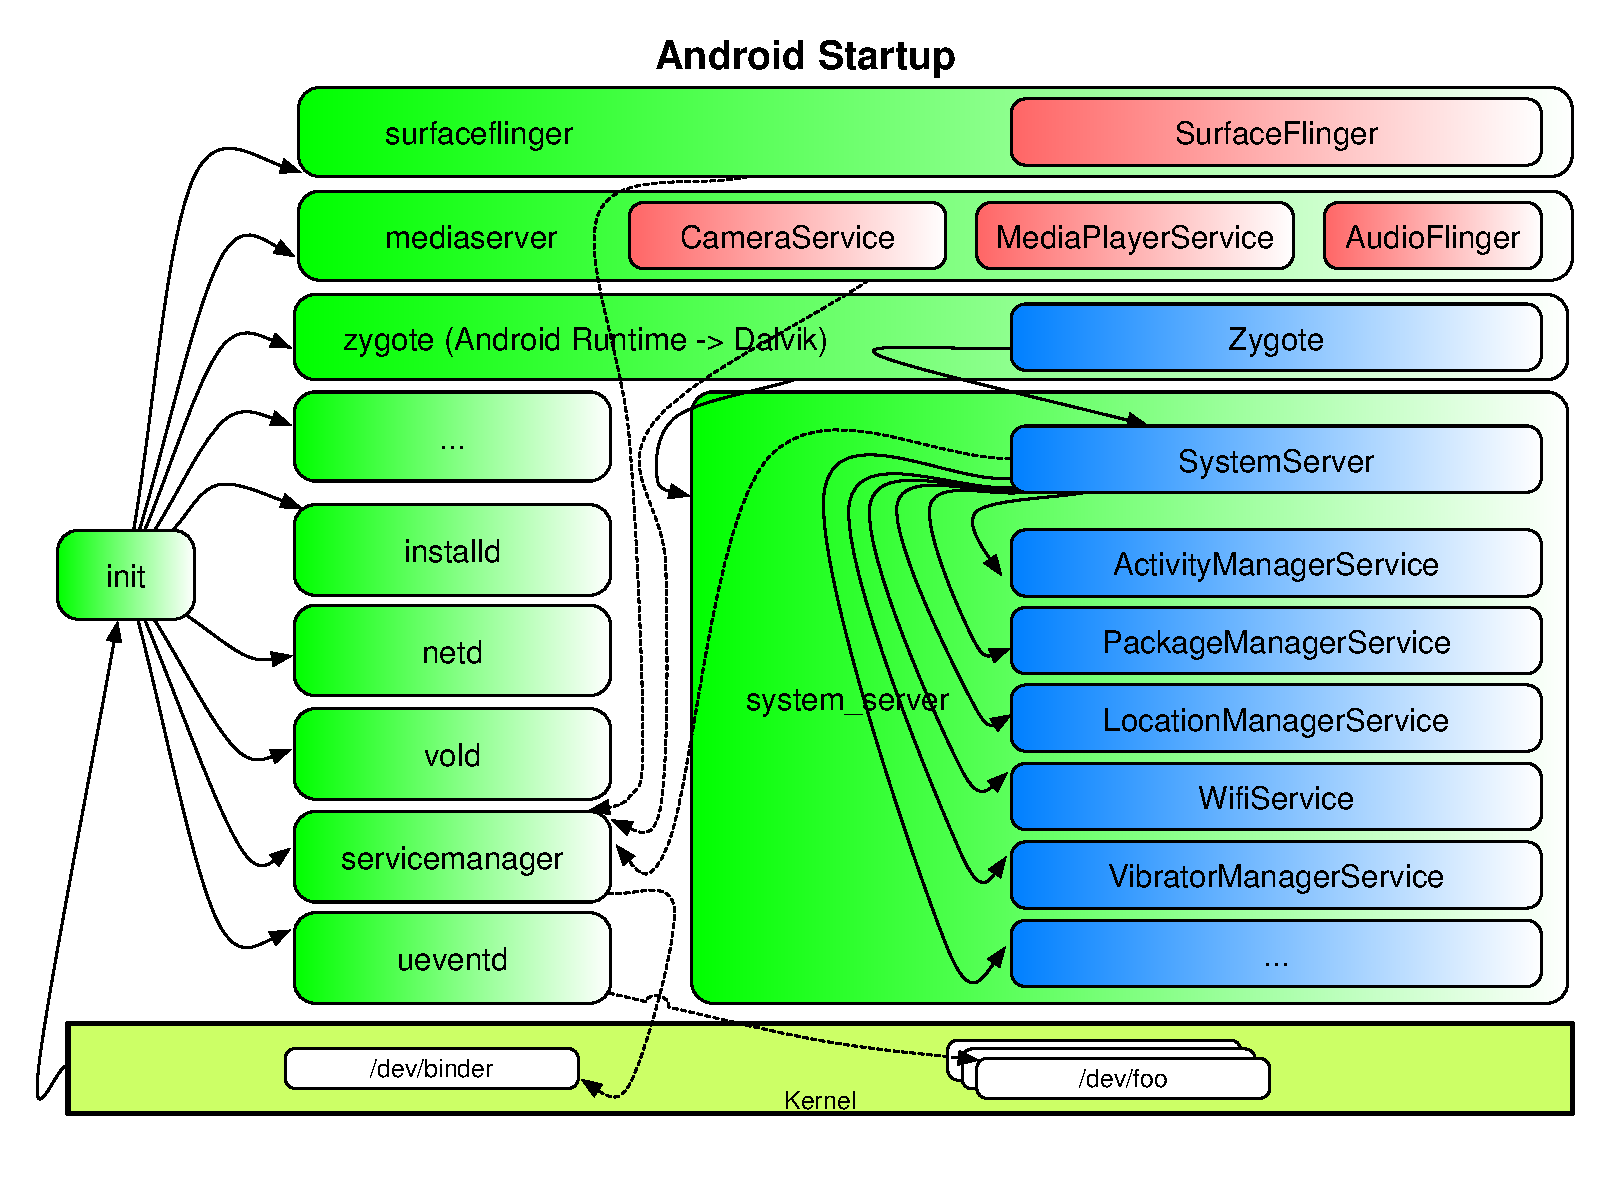
\includegraphics[scale=0.5]{img/marak/StartupWalkthru}
\caption{Schematizzazione della procedura di startup di Android. \parencite{site:marakAndroidInternals}}
\label{fig:marakStartup}
\end{figure}
Un'\textit{overview} generale dei processi che vengono attivati durante la procedura
di startup è fornita nella Figura \vref{fig:marakStartup}: mi
concentrerò sulla fase di attivazione del processo Zygote e del System Server, mentre
tratterò del Service Manager nella Sezione \vref{sec:ipcbinder}.

Un'importante differenza con i sistemi GNU/Linux è la presenza di un file
\texttt{\small init.rc} definito secondo un specifico linguaggio, detto \textsc{Android Init Language}
(descritto dal file riportato nella Sezione \vref{sec:appxINIT});
possiamo trovare il sorgente del file di inizializzazione al percorso:
\begin{center}
\AOSP\texttt{\small/system/core/rootdir/init.rc}
\end{center}
All'interno di questo file vengono effettuate, tra le altre, le seguenti operazioni:
\begin{itemize}
\diam Vengono inizializzate le variabili d'ambiente
\diam Viene effettuato il mounting delle varie componenti del \textit{filesystem}: è in questo punto dove, in particolare, si monta il \textit{root filesystem} e la cartella \texttt{\small /system} come di sola lettura.
\diam Vengono definite le proprietà di sistema tramite il comando \texttt{setprop}: tra gli altri parametri, figurano le configurazioni sui permessi utente della Shell, e la quantità di dati utilizzata all'interno dei buffer di sistema per la comunicazione TCP:
\begin{bash}
# Define TCP buffer sizes for various networks
#   ReadMin, ReadInitial, ReadMax, WriteMin, WriteInitial, WriteMax,
    setprop net.tcp.buffersize.default 4096,87380,110208,4096,16384,110208
    setprop net.tcp.buffersize.wifi    524288,1048576,2097152,262144,524288,1048576
    setprop net.tcp.buffersize.lte     524288,1048576,2097152,262144,524288,1048576
    setprop net.tcp.buffersize.umts    4094,87380,110208,4096,16384,110208
    setprop net.tcp.buffersize.hspa    4094,87380,262144,4096,16384,262144
    setprop net.tcp.buffersize.hsupa   4094,87380,262144,4096,16384,262144
    setprop net.tcp.buffersize.hsdpa   4094,87380,262144,4096,16384,262144
    setprop net.tcp.buffersize.hspap   4094,87380,1220608,4096,16384,1220608
    setprop net.tcp.buffersize.edge    4093,26280,35040,4096,16384,35040
    setprop net.tcp.buffersize.gprs    4092,8760,11680,4096,8760,11680
    setprop net.tcp.buffersize.evdo    4094,87380,262144,4096,16384,262144
\end{bash}
\diam Vengono avviati i \textit{service} di sistema con gli adeguati permessi e socket di comunicazione.
\end{itemize}


Tra gli altri \textit{service} viene iniziato Zygote tramite le seguenti istruzioni:
\begin{bash}
service zygote /system/bin/app_process -Xzygote /system/bin --zygote --start-system-server
    class main
    socket zygote stream 660 root system
    onrestart write /sys/android_power/request_state wake
    onrestart write /sys/power/state on
    onrestart restart media
    onrestart restart netd
\end{bash}
Possiamo quindi notare che \texttt{\small app\_process} all'interno del sorgente
è situato all'interno del file:
\begin{center}
\texttt{\small \d AOSP/frameworks/base/cmds/app\_process/app\_main.cpp}
\end{center}
che, come vediamo, ha il compito sia di eseguire Zygote, sia di eseguire
una qualsiasi classe Java che contenga al suo interno un metodo \texttt{\small main}.
In particolare tale esecuzione è garantita dalle funzioni di inizializzazione
della DVM, che sono descritte all'interno del file:
\begin{center}
\texttt{\small \AOSP/frameworks/base/core/jni/AndroidRuntime.cpp}
\end{center}

Come si può notare dal suo sorgente, è in questo luogo che avvengono le inizializzazioni
dello strato di interazione JNI, effettuando l'invocazione delle funzioni
descritte all'interno della variabile:
\begin{clang}
static const RegJNIRec gRecJNI = {
   ...  REG_JNI(funzione), ...
}
\end{clang}
Queste funzioni verranno invocate tramite l'esecuzione del metodo \texttt{\small start},
che a sua volta invoca il metodo \texttt{\small startReg}, accettando come argomento
l'array mostrato sopra. All'interno di quest'ultimo compare anche il riferimento
alla funzione \texttt{\small register\_android\_os\_Binder} che, definita tra le componenti
del Binder lato JNI, richiama a sua volta le funzioni:
\begin{itemize}
\item \texttt{\small int\_register\_android\_os\_Binder}
\item \texttt{\small int\_register\_android\_os\_BinderInternal}
\item \texttt{\small int\_register\_android\_os\_BinderProxy}
\end{itemize}

\textit{A questo punto posso notare come la necessità della definizione di una 
nuova macchina virtuale sia dettata, più che per motivi di efficienza e 
di implementazione come viene mostrato in \parencite[9-11]{libro:carli}, 
dalla necessità di consentire le inizializzazioni dello strato JNI utilizzate
dai \textrm{service} Java del sistema operativo. }

Passando quindi alla funzione di inizializzazione \texttt{\small int\_register\_android\_os\_Binder},
posso notare come venga inizializzata la variabile \texttt{\small gBinderOffsets}
definita all'interno del file per la configurazione del Binder lato JNI, effettuando
all'interno dei campi della struttura che essa rappresenta le seguenti associazioni:
\begin{description}
\item[\texttt{\small mClass}] ottiene un riferimento alla classe Java \texttt{\small Binder}
\item[\texttt{\small mExecTransact}] ottiene il riferimento al metodo \texttt{\small execTransact} della
	classe di cui sopra.
\item[\texttt{\small mObject}] mentre nella classe Java corrispondente questo corrisponderà
	ad un intero, lato JNI rappresenterà il puntatore ad un oggetto nativo
	di tipo \texttt{\small JavaBBinderHolder}.
\end{description}
All'interno della stessa funzione JNI, si procede alla registrazione dei 
metodi nativi definiti in \texttt{\small gBinderMethods}.

Viene quindi eseguita la classe descritta dal file:\\
\texttt{\small \AOSP/frameworks/base/core/java/com/android/internal/os/ZygoteInit.java}

Dalla funzione \texttt{\small main} ivi definita viene quindi avviato il System
Server, descritto dal file:\\
\texttt{\small \AOSP/frameworks/base/services/java/com/android/server/SystemServer.java}

Possiamo vedere come da lato Java si esegua il metodo nativo \texttt{\small init1()}
definito all'interno del file:\\
\texttt{\small \AOSP/frameworks/base/services/jni/com\_android\_server\_SystemServer.cpp}

E, dalla cui definizione, si effettua l'esecuzione del metodo \texttt{\small system\_init()},
definito all'interno della libreria \texttt{\small system\_service} ed in particolare 
per il file:\\
\texttt{\small \AOSP/frameworks/base/cmds/system\_server/library/system\_init.cpp}

in questo luogo, subito dopo aver lanciato il metodo nativo all'interno della
macchina virtuale, si entra all'interno del \textit{main loop} per la raccolta
di richieste da parte delle applicazioni in esecuzione
nel sistema.


Questo poi si preoccupa di inizializzare, tra gli altri, i seguenti gestori lato
Java all'interno del metodo \texttt{\small init2()}:
\begin{itemize}
\diam \texttt{\small DevicePolicyManagerService}
\diam \texttt{\small NetworkManagementService}
\diam \texttt{\small ConnectivityService}
\diam \texttt{\small ThrottleService}
\diam \texttt{\small AudioService}
\end{itemize}
Una lista completa dei servizi in esecuzione all'interno del dispositivo è 
fornita eseguendo l'istruzione \texttt{\small service list} via terminale del 
dispositivo Android. Tuttavia non è presente una sufficiente documentazione
di come questi servizi interagiscano \parencite{libro:embedded}: lo studio dei
vari errori durante i tentativi di porting di \texttt{\small pjsua} possono costituire
 l'occasione per effettuare una prima indagine.

\section{Differenze tra Bionic e Libc}\label{sec:diffbilib}
Analizzando la computazione di \texttt{\small strace} dall'emulatore, possiamo osservare
come, all'interno di un sistema operativo Andorid, avvengano molte più chiamate
a systemcall rispetto all'esecuzione dello stesso binario all'interno di un 
computer con sistema operativo GNU/Linux. Tra queste possiamo notare la seguente:
\begin{center}
\texttt{\small open("/dev/urandom", O\_RDONLY|O\_LARGEFILE)}
\end{center}
L'apertura del \textit{device} in questione fa riferimento alla generazione di valori 
Random: tramite questo \textit{device}, il sistema operativo si assicura che, i 
numeri casuali generati, siano sempre crittograficamente sicuri. Possiamo notare
quindi che la libreria \textit{Bionic} di Google è stata scritta appositamente
per utilizzare le peculiarità del sistema operativo Andorid, che lo differenziano
da GNU/Linux.

Un'ulteriore differenza tra queste due librerie è provato dall'utilizzo del
driver \texttt{\small ashmem} per effettuare la creazione di aree di memoria
condivise tra processi: questa implementazione presenta delle API simili a quelle
POSIX per, anche se dopo aver ottenuto un \textit{file descriptor} dal driver
è necessario effettuarne il \texttt{\small mmap}, come illustrato dall'esempio
proposto di seguito:
\begin{clang}
#define MAX 4096
#define NAME "regione"
void* data;
int fd = ashmem_create_region(NAME,MAX);
if (fd<=0) return;
if (data = mmap(NULL,MAX,PROT_READ|PROT_WRITE,MAP_SHARED,fd,0)) {
	/* no further ancillary data is provided */
}
\end{clang}
Questo device è utilizzato allo scopo di garantire la liberazione della memoria
condivisa da parte del Kernel \parencite{site:marakAndroidInternals}. 
È anche utilizzata, come mostrerò in seguito, per permettere la comunicazione 
diretta tra due thread.

Un ulteriore differenza di implementazione è costituita dall'implementazione
dei thread, che è inclusa direttamente all'interno della libreria \textit{Bionic}:
per la compilazione di sorgente che utilizza thread non è quindi necessario
effettuare il linking con una libreria \texttt{\small pthread}.


